\documentclass[14pt,pdf,utf8,russian,aspectratio=169,hyperref={unicode}]{beamer}
\usepackage{amsmath, bm}
\usepackage[T2A]{fontenc}
\usepackage[russian, english]{babel}
\usepackage[export]{adjustbox}
\usepackage{wrapfig}
\usepackage{soul}
\usepackage[normalem]{ulem}

\title{Sample Title}
\subtitle{Sample Subtitle}

\usetheme{lucid}
\begin{document}
    \frame {
      \vskip0.4cm
       \begin{columns}[t] % contents are top vertically aligned
         \begin{column}[c]{.4\textwidth} % each column can also be its own environment
           
\includegraphics[width=3cm, right]{logo/bb1.png}
         \end{column}
         \begin{column}[c]{.6\textwidth}
           {
           %\vspace{10pt}
           {\Large\bf\textcolor{bb-green}{Building}\textcolor{ap-b}{Blocks}}
           \\
           {\normalsize \hspace{2pt} Pavel Botov}
           }
         \end{column}
       \end{columns}
        }
\frame {
	    \frametitle{Content}
	    \begin{itemize}
	      \pause\item Теорминимум
          \pause\item Эксперимент
          \pause\item Нежданности          
        \end{itemize}
    }
\frame {
        \frametitle{Теоретический минимум}
	    \framesubtitle{What is {\bf file}?}
	    Файл имеет:
        \begin{itemize}
          \pause\item {\bf inode}. Но про это пока говорить рано
          \pause\item {\bf имя}. Может быть, несколько. Или ни одного. Но это нам сейчас не интересно
          \pause\item прочие {\bf метаданные}. Но нам это сейчас не интересно          
          \pause\item {\bf тело} (или {\bf содержимое}, или {\bf content})
        \end{itemize}
    }
\frame {
        \frametitle{Теоретический минимум}
	    \framesubtitle{What is {\bf file content}?}
	    Тело файла:
        \begin{itemize}
          \pause\item имеет {\bf размер}, который можно менять (в любую сторону)
          \pause\item можно {\bf читать} с любой позиции (иногда даже вне рамок${}^{*}$)
          \pause\item можно {\bf писать} в любую позицию и дописывать в конец
          \pause\item нельзя${}^{*}$ {\bf сдвигать}, {\bf объединять} с другим телом
        \end{itemize}
    }
\frame {
	\frametitle{Теоретический минимум}
	\framesubtitle{What is file in {\bf file system}?}
	Файловая система организует хранение файлов на блочном устройстве.\\
	\vspace{0.4cm}
	В файловой системе:
	\begin{itemize}
		\pause\item Метаданные файла хранятся отдельно от тела,\\ но это \sout{не точно} не всегда         
		\pause\item На тело выделяется целое число блоков
		\pause\item Начало тела файла выровнено по началу блока
		\pause\item Кроме метаданных и тела есть ещё кое что...
	\end{itemize}
}
\frame {
	\frametitle{Теоретический минимум}
	\framesubtitle{Файл и фрагментация}
	
	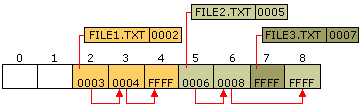
\includegraphics[width=0.5\linewidth, center]{pics/31fat.png}
	\pause Чаще всего тело файла располагается на последующих друг за другом блоках.	
	\pause Но иногда оно занимает несколько таких последовательностей - {\bf фрагментов}.
}
\frame {
	\frametitle{Теоретический минимум}
	\framesubtitle{Происхождение фрагментации}
	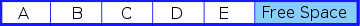
\includegraphics[width=0.5\linewidth, center]{pics/frags-1.png}\\
	\hspace{1cm} Файлы A, B, C, D и E и ещё места осталось...
}
\frame {
	\frametitle{Теоретический минимум}
	\framesubtitle{Происхождение фрагментации}
	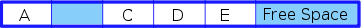
\includegraphics[width=0.5\linewidth, center]{pics/frags-2.png}\\
	\hspace{1cm}Файл B удалили. Появилась "дырка"
}
\frame {
	\frametitle{Теоретический минимум}
	\framesubtitle{Происхождение фрагментации}
	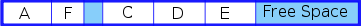
\includegraphics[width=0.5\linewidth, center]{pics/frags-3.png}\\
	\hspace{1cm}Записали новый небольшой файл F.\\
	\pause\hspace{1cm}Он занял эту дырку. Но не всю.
}
\frame {
	\frametitle{Теоретический минимум}
	\framesubtitle{Происхождение фрагментации}
	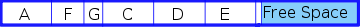
\includegraphics[width=0.5\linewidth, center]{pics/frags-5.png}\\
	\hspace{1cm}Записали новый файл G.\\
	\pause\hspace{1cm}Он занял остаток дырки и...\\
	\pause\hspace{2cm}... отъел ещё свободного пространства.
}

\frame {
	\frametitle{Теоретический минимум}
	\framesubtitle{Файловые системы}
	\pause Я помню много всяких их:
	\begin{itemize}
		\pause\item FAT32/FAT16/FAT12
		\pause\item ext2/ext3/ext4
		\pause\item Reiser3/ReiserFS
		\pause\item XFS
		\pause\item BTRFS
		\pause\item exFAT
		\pause\item ReFS
		\pause\item NTFS
	\end{itemize}
	\pause Вот на последней и остановимся
}
\frame {
	\frametitle{Теоретический минимум}
	\framesubtitle{Хранение файла в NTFS}
	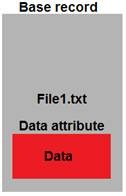
\includegraphics[width=0.2\linewidth, center]{pics/ntfs1.jpg}\\
	{\bf Base record} хранит метаданные и само тело файла.
	\vspace{0.5cm}
	\begin{center}
		\tiny\url{https://docs.microsoft.com/ru-ru/archive/blogs/askcore/the-four-stages-of-ntfs-file-growth-part-2}
	\end{center}
}
\frame {
	\frametitle{Теоретический минимум}
	\framesubtitle{Хранение файла в NTFS}
	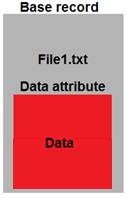
\includegraphics[width=0.2\linewidth, center]{pics/ntfs2.jpg}\\
	Файл растёт, но умещается в {\bf Base record}
}
\frame {
	\frametitle{Теоретический минимум}
	\framesubtitle{Хранение файла в NTFS}
	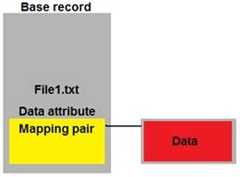
\includegraphics[width=0.3\linewidth, center]{pics/ntfs3.jpg}\\
	Файл растёт. Тело уже не умещается в {\bf Base record} и выносится наружу в отдельный {\bf фрагмент}.
}
\frame {
	\frametitle{Теоретический минимум}
	\framesubtitle{Хранение файла в NTFS}
	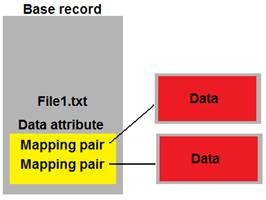
\includegraphics[width=0.3\linewidth, center]{pics/ntfs4.jpg}\\
	Фрагментов уже больше одного. Их позиции и длины хранятся в {\bf Base record}
}
\frame {
	\frametitle{Теоретический минимум}
	\framesubtitle{Хранение файла в NTFS}
	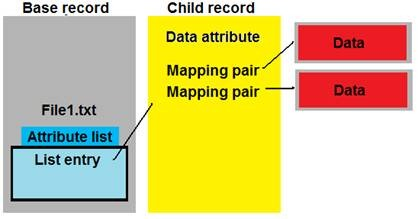
\includegraphics[width=0.4\linewidth, center]{pics/ntfs5.jpg}\\
	Фрагментов так много, что они не помещаются в {\bf Base record}. Под них заводится отдельнынй блок {\bf Child record }
}
\frame {
	\frametitle{Теоретический минимум}
	\framesubtitle{Хранение файла в NTFS}
	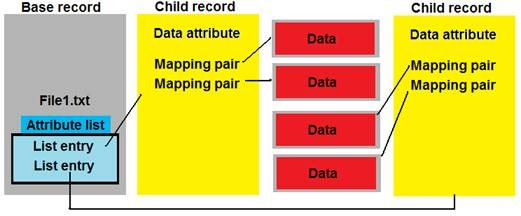
\includegraphics[width=0.5\linewidth, center]{pics/ntfs6.jpg}\\
	Расщепляем {\bf Child record }
}
\frame {
	\frametitle{Теоретический минимум}
	\framesubtitle{Хранение файла в NTFS}
	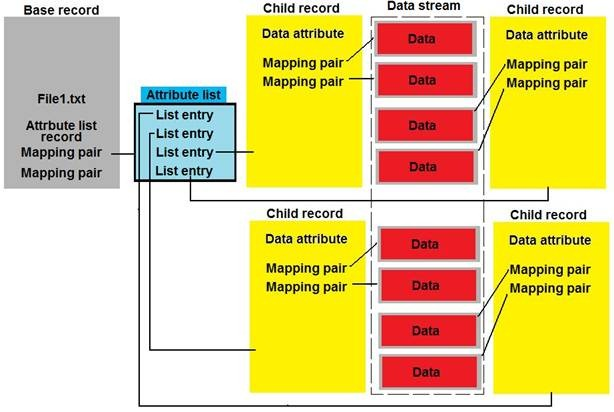
\includegraphics[width=0.5\linewidth, center]{pics/ntfs7.jpg}\\
	Продолжаем плодить сущностей по мере необходимости...\\
	\pause Для NTFS {\bf это предел}: 3 уровня узлов для хранения ссылок на все фрагменты.
}
\frame {
	\frametitle{Эксперимент}
	\framesubtitle{На что смотрим-то?}
	\pause \large{Вопрос 1: Как быстрее записывать большой файл?}\\
	\pause \large{Вопрос 2: A это потом влияет на скорость чтения?}
}
\frame {
	\frametitle{Эксперимент}
	\framesubtitle{Как пишем?}
	\begin{itemize}	
		\pause\item Пишем сразу два одинаковых файла одинаковым  образом
		\pause\item Сценарии записи:
		\begin{enumerate}
			\pause\item Просто пишем в файл\\
			\visible<4->{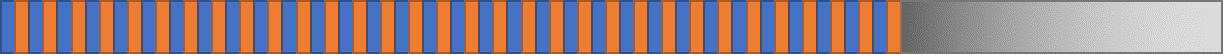
\includegraphics[width=0.75\linewidth, center]{pics/scenario1.png}}
			\pause\item Заранее выделим место и далее пишем\\
			\visible<5->{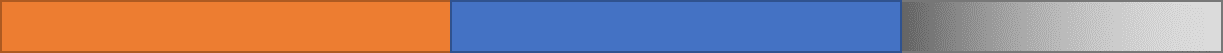
\includegraphics[width=0.75\linewidth, center]{pics/scenario2.png}}
			\pause\item Ресайзим файл в два раза по мере наполнения\\
			\visible<6->{
\includegraphics[width=0.75\linewidth, center]{pics/scenario3.png}}
		\end{enumerate}
		\pause\item Замеряем время от создания файла до последнего flush'а
		\pause\item Делаем 20 итераций, старые файлы не удаляем
	\end{itemize}
}
\frame {
	\frametitle{Эксперимент}
	\framesubtitle{Как читаем?}
	\begin{itemize}
		\pause\item Читаем {\bf два байта}:
		\begin{enumerate}
			\pause\item либо в центре блока
			\visible<3->{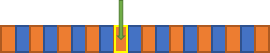
\includegraphics[width=0.45\linewidth, center]{pics/read1.png}}
			\pause\item либо на границе двух блоков
			\visible<4->{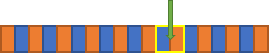
\includegraphics[width=0.45\linewidth, center]{pics/read2.png}}
		\end{enumerate}
		\pause\item Никакие два блока не читаются больше одного раза
		\pause\item Читаем файлы в порядке их появления
		\pause\item Делалось 5000 случайных замеров на файл, крайние 1000 отбрасывались, результат усреднялся
	\end{itemize}
}
\frame {
	\frametitle{Эксперимент}
	\framesubtitle{Стенд}
	\begin{itemize}
		\item {\bf HDD}: Seagate 8TB, 256MiB cache, SATA300 {\small (ST8000VN0002)}
		\item {\bf FS}: NTFS, 4K-block, Win10, 90\% free
		\item {\bf Rintime}: .Net Core v3.1
	\end{itemize}
	Всего делалось 20 итераций. Размер файлов - по 4ГБ.
}
\frame {
	\frametitle{Эксперимент}
	\framesubtitle{Результаты: число фрагментов}
	
	Итоговое число фрагментов в файле:
		\begin{enumerate}
			\pause\item Просто пишем в файл - {\bf 65539} (что меньше 1М в 16 раз!)
			\pause\item Заранее выделим место - {\bf 1} (согласно теории)
			\pause\item Ресайзим файл - {\bf 21} (согласно теории)
		\end{enumerate}
}
\frame {
	\frametitle{Эксперимент}
	\framesubtitle{Результаты: скорость записи}
	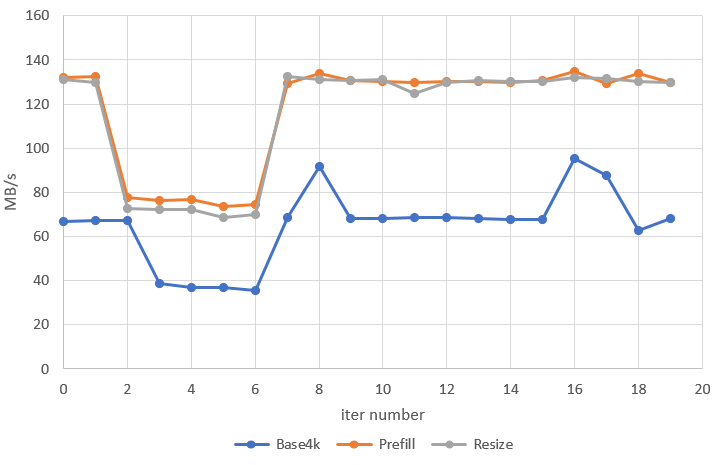
\includegraphics[width=0.65\paperwidth, center]{pics/write-results.png}
}
\frame {
	\frametitle{Эксперимент}
	\framesubtitle{Результаты: скорость записи}
	\begin{columns}
		\begin{column}[c]{0.45\paperwidth}
			И что мы видим?
			\begin{itemize}
					\pause\item Необъяснимые провалы!\\И они сохраняются
					\pause\item Base4k медленнее в 2 раза!
					\pause\item Prefill чуть быстрее Resize
				\end{itemize}
		\end{column}
		\begin{column}[c]{0.5\paperwidth}
			\begin{minipage}[c]{1\textwidth}
				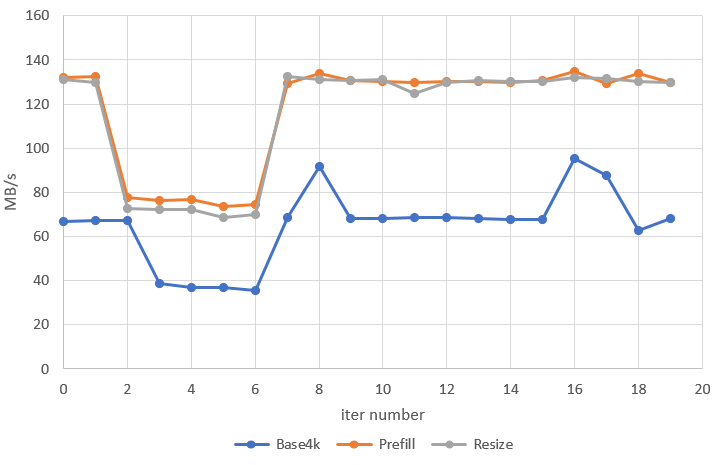
\includegraphics[width=\textwidth]{pics/write-results.png}
			\end{minipage}
		\end{column}
	\end{columns}
}
\frame {
	\frametitle{Эксперимент}
	\framesubtitle{Результаты: время {\bf случайного} чтения}
	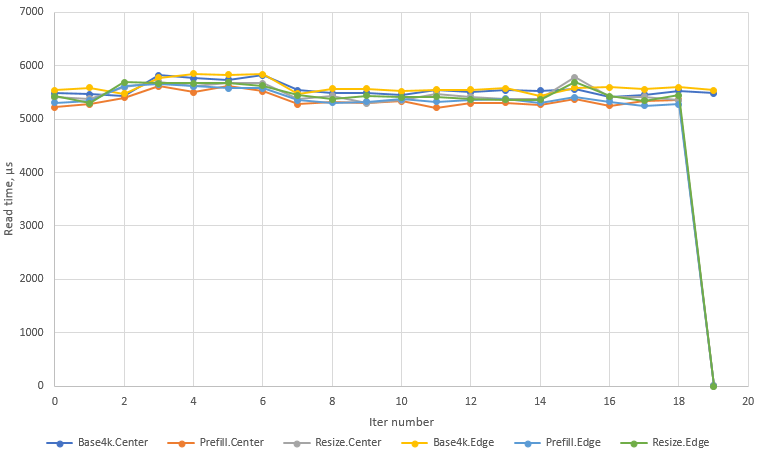
\includegraphics[width=0.7\paperwidth, center]{pics/read-results.png}
}
\frame {
	\frametitle{Эксперимент}
	\framesubtitle{Результаты: время {\bf случайного} чтения}
	\begin{columns}
		\begin{column}[c]{0.5\paperwidth}
			\begin{minipage}[c]{1\textwidth}
				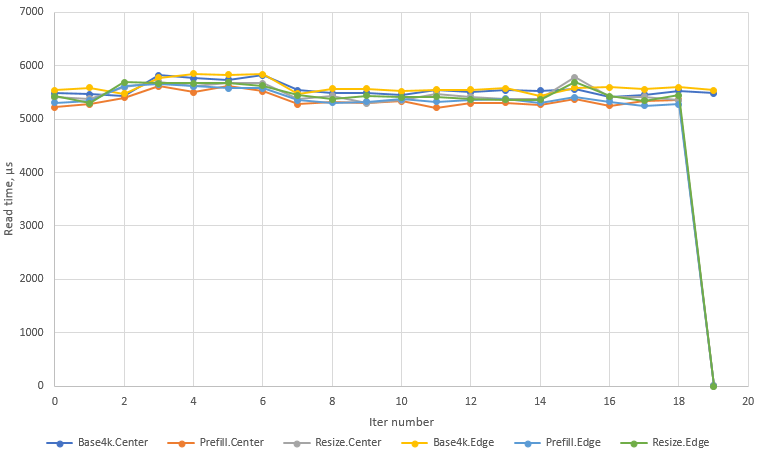
\includegraphics[width=\textwidth]{pics/read-results.png}
			\end{minipage}
		\end{column}
		\begin{column}[c]{0.45\paperwidth}
			\begin{minipage}[c]{1\textwidth}
				И что мы видим?
				\begin{itemize}
					\pause\item Последние 16ГБ файлов читались из кэша OS
					\pause\item Center быстрее edge не более чем на 1\%
					\pause\item Base4k самый медленный, Prefill самый быстрый, но разница не более 1\%
				\end{itemize}
			\end{minipage}
		\end{column}
	\end{columns}
}
\frame {
	\frametitle{Эксперимент}
	\framesubtitle{Результаты: время {\bf линейного} чтения}
	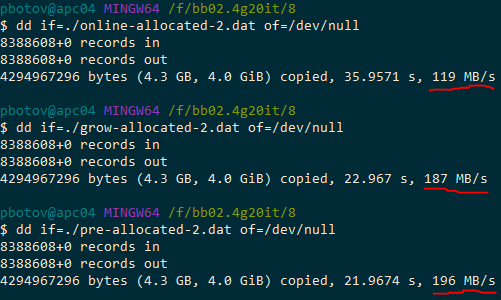
\includegraphics[width=0.55\paperwidth, center]{pics/read-linear.png}
	\begin{center}
	Чтение фрагментированного файла заметно дольше
	\end{center}
}
\frame {
	\frametitle{Нежданчик}
	\framesubtitle{Шлейф постзаписи}
	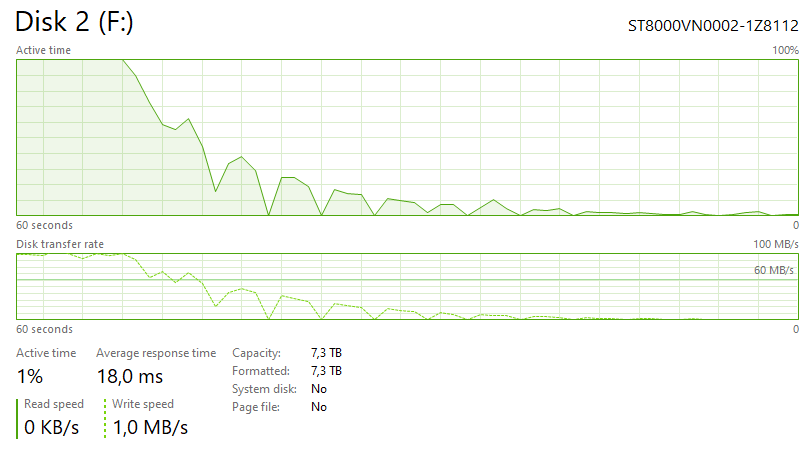
\includegraphics[width=0.65\linewidth, center]{pics/tail.png}\\
	После прогона каждого сценария приходилось делать паузу на две минуты. Запись на диск продолжается ещё некоторое время!
}
\frame {
	\frametitle{Жданчик}
	\begin{center}
	\bf\large\emph{System.IO.IOException: The requested operation could not be completed due to a file system limitation}
	\end{center}
	\pause - такое исключение можно словить в первом сценарии, если размер файла не ограничивать в 4ГБ, и продолжить запись до \sout{8ТБ} до 151ГБ.
}
\frame {
	\frametitle{Жданчик}
	Разгадаем ребус:
	\vspace{0.1cm}
	\begin{columns}
		\begin{column}[c]{0.4\paperwidth}
			\begin{minipage}[c]{1\textwidth}
				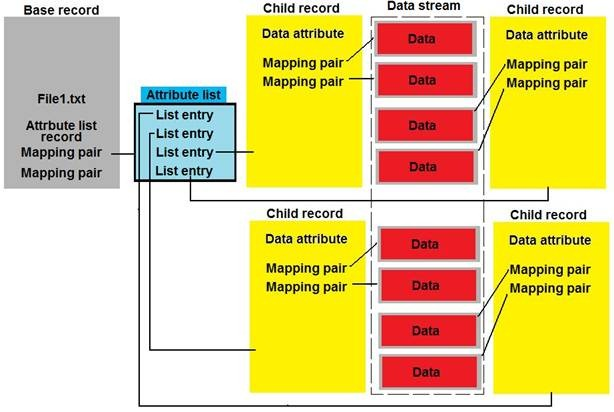
\includegraphics[width=\textwidth]{pics/ntfs7.jpg}
			\end{minipage}
		\end{column}
		\begin{column}[c]{0.6\paperwidth}
			\begin{minipage}[c]{1\textwidth}
				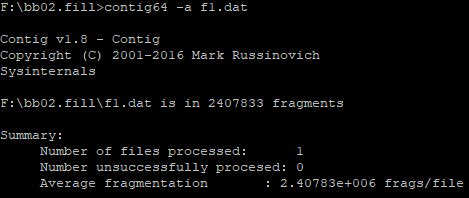
\includegraphics[width=\textwidth]{pics/contig64.png}
			\end{minipage}
		\end{column}
	\end{columns}
}
\frame {
	\frametitle{Жданчик}
	Разгадаем ребус:
	\vspace{0.1cm}
	\begin{columns}
		\begin{column}[c]{0.317\paperwidth}
			\begin{minipage}[c]{1\textwidth}
				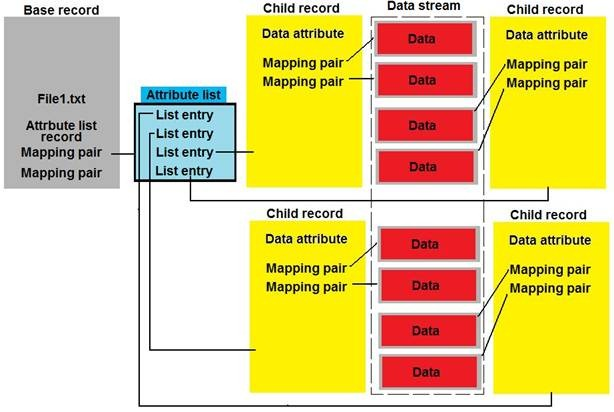
\includegraphics[width=\textwidth]{pics/ntfs7.jpg}
			\end{minipage}
		\end{column}
		\begin{column}[c]{0.502\paperwidth}
			\begin{minipage}[c]{1\textwidth}
				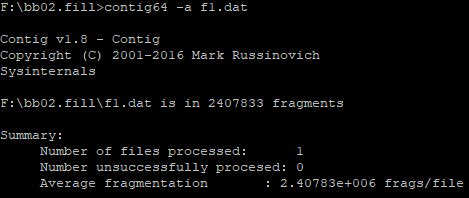
\includegraphics[width=\textwidth]{pics/contig64.png}
			\end{minipage}
		\end{column}
	\end{columns}
	\vspace{0.1cm}
	\begin{itemize}
	\pause\item NTFS имеет ограничение на число фрагментов на файл
	\pause\item В нашем случае $\approx$ 2.4М фрагментов
	\pause\item Проявлялось год назад при записи в ARC на проде
	\pause\item NBlob этой проблемой не страдает by design. :)
	\end{itemize}
}
\frame {
	\frametitle{Выводы}
	\begin{enumerate}
		\pause\item Большим файлам особый уход. Если есть возможность, выделяйте место заранее
		\pause\item Скорость линейного чтения фрагментированного файла значительно ниже. Случайное - не особо
		\pause\item Последние записанные файлы хранятся в кэше MS Windows и доступны на чтение
		\pause\item Реальный минимальный размер фрагмента в NTFS оказался 64КБ${}^{*}$
		\pause\item \sout{Тестировать производительность сложно} Всё сложно
		\pause\item \LaTeX -презенташки можно делать и под windows
	\end{enumerate}
}
\frame {
	\begin{center}
		\vspace{2cm}
		\large\href{https://github.com/antiplagiat/BuildingBlocks}{https://github.com/antiplagiat/\textcolor{bb-green}{Building}\textcolor{ap-b}{Blocks}}\\
	\end{center}
}
\end{document}
